\documentclass{beamer}
\usepackage{amsmath}
\usepackage{amssymb}
\usepackage{graphicx}

\usetheme{default} % Or any other Beamer theme
\usefonttheme{serif} 

\title{Mathematical Description of Shape Changes in Solids}
\author{Your Name}
\date{\today}

\begin{document}

\begin{frame}
  \titlepage
\end{frame}

\begin{frame}{Introduction}
  \begin{itemize}
    \item   The purpose of this chapter is to summarize the equations that govern the response of solids to mechanical or thermal loading.
    \item   We will focus on the mathematical description of shape changes in a solid.
    \item   This includes displacement and velocity fields, and deformation gradient tensors.
  \end{itemize}
\end{frame}

\begin{frame}{Mathematical description of shape changes in solids}
    \begin{itemize}
        \item   In this section, we list the various mathematical formulas that are used to characterize shape changes in solids (and in fluids).
        \item   The formulas might look scary at first, but they are mostly just definitions.
        \item   Shape changes near a point can always be characterized by six numbers.
    \end{itemize}
\end{frame}

\begin{frame}{Mathematical description of shape changes in solids (continued)}
    \begin{itemize}
        \item   These could be the six independent components of the Lagrangian strain, Eulerian strain, the left or right stretch tensors, or your own favorite deformation measure.
        \item   Given the complete set of six numbers for any one deformation measure, you can always calculate the components of other strain measures.
        \item   The reason that so many different deformation measures exist is partly that different material models adopt different strain measures, and partly because each measure is useful for describing a particular type of shape change.
    \end{itemize}
\end{frame}

\begin{frame}{The Displacement and Velocity Fields}
  \begin{itemize}
    \item   The displacement vector $\mathbf{u}(\mathbf{x}, t)$ describes the motion of each point in the solid.
    \item   The displacement vector is defined as:
    $$ \mathbf{y} = \mathbf{x} + \mathbf{u}(\mathbf{x}, t) $$
    \item   In index notation:
    $$ y_{i}=x_{i}+u_{i}(x_{1},x_{2},x_{3},t) $$
    \item   The displacement field completely specifies the change in shape of the solid.
  \end{itemize}
\begin{center}
   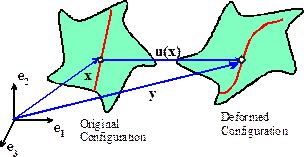
\includegraphics[width=0.6\textwidth]{../pictures/2-3/image004.png} 
\end{center}

\end{frame}

\begin{frame}{Velocity Field}
  \begin{itemize}
    \item   The velocity field describes the motion of the solid.
    \item   The velocity field is defined as the time derivative of the displacement field:
    $$ v_{i}(x_{k},t)=\frac{\partial y_{i}}{\partial t}=\frac{\partial u_{i}(x_{k},t)}{\partial t} \quad \text{x = const} $$
  \end{itemize}
\end{frame}

\begin{frame}{Examples of Simple Deformations}
  \begin{itemize}
    \item   \textbf{Volume preserving uniaxial extension}
    $$
    \begin{aligned}
      y_{1} &= \lambda x_{1} \\
      y_{2} &= x_{2} / \sqrt{\lambda} \\
      y_{3} &= x_{3} / \sqrt{\lambda}
    \end{aligned}
    $$

  \end{itemize}
\begin{center}
   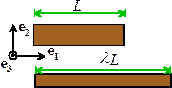
\includegraphics[width=0.5\textwidth]{../pictures/2-3/image008.png} 
\end{center}
\end{frame}

\begin{frame}{Examples of Simple Deformations}
  \begin{itemize}
    \item   \textbf{Simple shear}
    $$
    \begin{aligned}
      y_{1} &= x_{1} + \tan(\theta) x_{2} \\
      y_{2} &= x_{2} \\
      y_{3} &= x_{3}
    \end{aligned}
    $$
  \end{itemize}
\begin{center}
   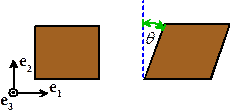
\includegraphics[width=0.5\textwidth]{../pictures/2-3/image011.png} 
\end{center}
\end{frame}

\begin{frame}{Examples of Simple Deformations (continued)}
  \begin{itemize}
    \item   \textbf{Rigid rotation through angle \(\theta\) about \(e_3\) axis}
    $$
    \begin{aligned}
      y_{1} &= x_{1} \cos(\theta) - x_{2} \sin(\theta) \\
      y_{2} &= x_{2} \cos(\theta) + x_{1} \sin(\theta) \\
      y_{3} &= x_{3}
    \end{aligned}
    $$
  \end{itemize}
  \begin{center}
   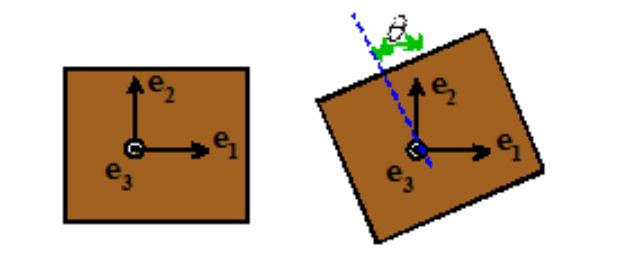
\includegraphics[width=0.5\textwidth]{../pictures/2-3/rigid-rot.png} 
\end{center}
\end{frame}

\begin{frame}{Examples of Simple Deformations (continued)}
  \begin{itemize}
    \item   \textbf{General rigid rotation about the origin}
    $$ \mathbf{y} = \mathbf{R} \cdot \mathbf{x} \quad \text{or} \quad y_{i_{r}}=R_{ij}x_{j} $$
    where \(\mathbf{R}\) must satisfy \(\mathbf{R} \cdot \mathbf{R}^T = \mathbf{R}^T \cdot \mathbf{R} = \mathbf{I}\) and \(\det(\mathbf{R}) > 0\) (\(\mathbf{R}\) is proper orthogonal). \(\mathbf{I}\) is the identity tensor
    with components
    $$
    \delta_{ik}=\begin{cases}
      1, & i=k \\
      0, & i \ne k
    \end{cases}
    $$
  \end{itemize}
  \begin{center}
   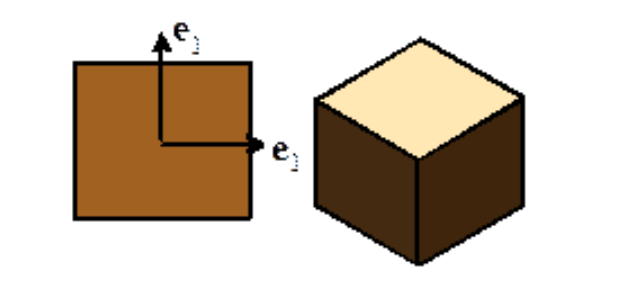
\includegraphics[width=0.5\textwidth]{../pictures/2-3/gen-rigid-rot.png} 
\end{center}
\end{frame}

\begin{frame}{Examples of Simple Deformations (continued)}
  \begin{itemize}
    \item   \textbf{General rigid rotation about the origin}
    Alternatively, a rigid rotation through angle \(\theta\) (with right hand screw convention) about an axis through the origin that is parallel to a unit vector \(\mathbf{n}\) can be written as
    $$ \mathbf{y} = \cos\theta \mathbf{x} + (1 - \cos\theta)(\mathbf{n} \cdot \mathbf{x})\mathbf{n} + \sin\theta (\mathbf{n} \times \mathbf{x}) $$
    \item   The components of R are thus
    $$ R_{ij} = \cos\theta \delta_{ij} + (1 - \cos\theta)n_i n_j + \sin\theta \epsilon_{ikj} n_k $$
    where \(\epsilon_{ijk}\) is the permutation symbol, satisfying
    $$
    \epsilon_{ijk}=\begin{cases}
      1 & i,j,k = 1,2,3; \quad 2,3,1 \text{ or } 3,1,2 \\
      -1 & i,j,k = 3,2,1; \quad 2,1,3 \text{ or } 1,3,2 \\
      0 & \text{otherwise}
    \end{cases}
    $$
  \end{itemize}
\end{frame}

\begin{frame}{Examples of Simple Deformations (continued)}
  \begin{itemize}
    \item   \textbf{General homogeneous deformation}
    $$
    \begin{aligned}
      y_1 &= A_{11} x_1 + A_{12} x_2 + A_{13} x_3 + c_1 \\
      y_2 &= A_{21} x_1 + A_{22} x_2 + A_{23} x_3 + c_2 \\
      y_3 &= A_{31} x_1 + A_{32} x_2 + A_{3} x_3 + c_3
    \end{aligned}
    $$
    or
    $$ \mathbf{y} = \mathbf{A} \cdot \mathbf{x} + \mathbf{c} \quad y_i = A_{ij} x_j + c_i $$
    where \(A_{ij}\) are constants.
    \item   The physical significance of a homogeneous deformation is that all straight lines in the solid remain straight under the deformation.
    \item   Thus, every point in the solid experiences the same shape change. All the deformations listed above are examples of homogeneous deformations.
  \end{itemize}
\end{frame}

\begin{frame}{Displacement Gradient Tensor}
    \begin{itemize}
        \item The displacement gradient tensor, denoted as \(\mathbf{u} \otimes \nabla\), is a second-order tensor.
        \item It is represented in component form as:
            \[
            \begin{bmatrix}
                \frac{\partial u_1}{\partial x_1} & \frac{\partial u_1}{\partial x_2} & \frac{\partial u_1}{\partial x_3} \\
                \frac{\partial u_2}{\partial x_1} & \frac{\partial u_2}{\partial x_2} & \frac{\partial u_2}{\partial x_3} \\
                \frac{\partial u_3}{\partial x_1} & \frac{\partial u_3}{\partial x_2} & \frac{\partial u_3}{\partial x_3}
            \end{bmatrix}
            \]
            where \(u_1\), \(u_2\), and \(u_3\) are the components of the displacement vector \(\mathbf{u}\), and \(x_1\), \(x_2\), and \(x_3\) are the components of the position vector \(\mathbf{x}\).
    \end{itemize}
\end{frame}

\begin{frame}{Deformation Gradient Tensor}
    \begin{itemize}
        \item The deformation gradient tensor, denoted as \(\mathbf{F}\), is a second-order tensor.
        \item It relates infinitesimal line elements in the undeformed and deformed configurations.
        \item It is defined as:
            \[
            \mathbf{F} = \mathbf{I} + \mathbf{u} \otimes \nabla
            \]
            where \(\mathbf{I}\) is the identity tensor, \(\mathbf{u}\) is the displacement vector, and \(\nabla\) is the gradient operator.
            \end{itemize}
            \end{frame}

\begin{frame}{Deformation Gradient Tensor}
\begin{itemize}
        \item In component form, this tensor is represented as:
            \[
            F_{ij} = \delta_{ij} + \frac{\partial u_i}{\partial x_j} = \frac{\partial y_i}{\partial x_j}
            \]
            or in matrix form:
            \[
            \begin{bmatrix}
                1 + \frac{\partial u_1}{\partial x_1} & \frac{\partial u_1}{\partial x_2} & \frac{\partial u_1}{\partial x_3} \\
                \frac{\partial u_2}{\partial x_1} & 1 + \frac{\partial u_2}{\partial x_2} & \frac{\partial u_2}{\partial x_3} \\
                \frac{\partial u_3}{\partial x_1} & \frac{\partial u_3}{\partial x_2} & 1 + \frac{\partial u_3}{\partial x_3}
            \end{bmatrix}
            =
            \begin{bmatrix}
                \frac{\partial y_1}{\partial x_1} & \frac{\partial y_1}{\partial x_2} & \frac{\partial y_1}{\partial x_3} \\
                \frac{\partial y_2}{\partial x_1} & \frac{\partial y_2}{\partial x_2} & \frac{\partial y_2}{\partial x_3} \\
                \frac{\partial y_3}{\partial x_1} & \frac{\partial y_3}{\partial x_2} & \frac{\partial y_3}{\partial x_3}
            \end{bmatrix}
            \]
            where \(u_i\) are the components of the displacement vector \(\mathbf{u}\), \(x_j\) are the components of the position vector \(\mathbf{x}\) in the undeformed configuration, \(y_i\) are the components of the position vector \(\mathbf{y}\) in the deformed configuration, and \(\delta_{ij}\) is the Kronecker delta.
    \end{itemize}
\end{frame}

\begin{frame}{Kronecker delta symbol}
    \begin{itemize}
        \item  The Kronecker delta symbol is defined as:
        $$
        \delta_{ik}=\begin{cases}
          1, & i=k \\
          0, & i \ne k
        \end{cases}
        $$
    \end{itemize}
\end{frame}

\begin{frame}{Displacement Gradient Tensor Continued}
  \begin{itemize}
    \item   Formally, the gradient of a vector field \(\mathbf{u}(\mathbf{x})\) is defined so that
    $$ [\mathbf{u} \otimes \nabla] \cdot \mathbf{n} = \lim_{\alpha \to 0} \frac{\mathbf{u}(\mathbf{x} + \alpha \mathbf{n}) - \mathbf{u}(\mathbf{x})}{\alpha} $$
    (for more details see Appendix B of https://solidmechanics.org/), but in practice the component formula \(\frac{\partial u_i}{\partial x_j}\) is more useful.
    \item   Note also that
    $$ \mathbf{y} \otimes \nabla = (\mathbf{x} + \mathbf{u}(\mathbf{x})) \otimes \nabla = \mathbf{F} $$
    or
    $$ \frac{\partial y_i}{\partial x_j} = \frac{\partial}{\partial x_j} (x_i + u_i) = \delta_{ij} + \frac{\partial u_i}{\partial x_j} = F_{ij} $$
    The rules of differentiation using index notation are described in more detail in Appendix C of https://solidmechanics.org/.
  \end{itemize}
  % Space for figure
\end{frame}

\begin{frame}{Deformation Gradient Tensor and Infinitesimal Line Elements}
  \begin{itemize}
    \item   The concepts of displacement gradient and deformation gradient are introduced to quantify the change in shape of infinitesimal line elements in a solid body.
    \item   Imagine drawing a straight line on the undeformed configuration of a solid.
    \item   The line would be mapped to a smooth curve on the deformed configuration.
  \end{itemize}

    \begin{center}
   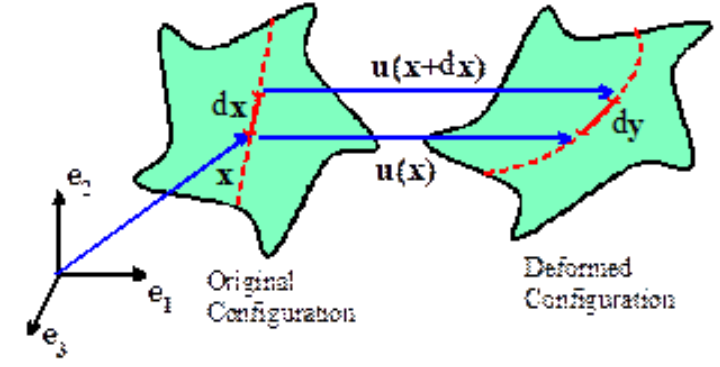
\includegraphics[width=0.5\textwidth]{../pictures/2-3/infinitesimal.png} 
\end{center}
  % Space for figure: Add figure illustrating line elements (e.g., Fig. 2.2 from the document)
\end{frame}

\begin{frame}{Deformation Gradient Tensor and Infinitesimal Line Elements}
  \begin{itemize}
    \item   Focus on a line segment dx, much shorter than the radius of curvature of this curve.
    \item   The segment would be straight in the undeformed configuration, and also (almost) straight in the deformed configuration.
    \item   Infinitesimal line segments are merely stretched and rotated by a deformation.
    \item   The infinitesimal line segments dx and dy are related by
    $$ dy = F \cdot dx \quad \text{or} \quad dy_i = F_{ik} dx_k $$
  \end{itemize}
  % Space for figure: Add figure illustrating line elements (e.g., Fig. 2.2 from the document)
\end{frame}

\begin{frame}{Deformation Gradient Tensor as a Matrix Equation}
    \begin{itemize}
        \item   Written out as a matrix equation, we have
        $$
        \begin{bmatrix}
          dy_1 \\
          dy_2 \\
          dy_3
        \end{bmatrix} =
        \begin{bmatrix}
          1 + \frac{\partial u_1}{\partial x_1} & \frac{\partial u_1}{\partial x_2} & \frac{\partial u_1}{\partial x_3} \\
          \frac{\partial u_2}{\partial x_1} & 1 + \frac{\partial u_2}{\partial x_2} & \frac{\partial u_2}{\partial x_2} \\
          \frac{\partial u_2}{\partial x_1} & \frac{\partial u_2}{\partial x_1} & \frac{\partial u_2}{\partial x_1}
        \end{bmatrix}
        \begin{bmatrix}
          dx_1 \\
          dx_2 \\
          dx_3
        \end{bmatrix}
        $$
    \end{itemize}
\end{frame}

\begin{frame}{Derivation of  dy = F · dx}
  \begin{itemize}
    \item   Consider an infinitesimal line element dx in a deforming solid.
    \item   When the solid is deformed, this line element is stretched and rotated to a deformed line element dy.
    \item   If we know the displacement field in the solid, we can compute \(dy = [x + dx + u(x + dx)] - [x + u(x)]\) from the position vectors of its two endpoints.
    \item   Expand \(u_{i}(x_{k}+dx_{k})\) as a Taylor series
    $$ u_{i}(x_{k}+dx_{k}) \approx u_{i}(x_{k})+\frac{\partial u_{i}}{\partial x_{k}}dx_{k} $$
    so that
    $$ dy_{i}=x_{i}+dx_{i}+u_{i}(x_{k}+dx_{k})-(x_{i}+u_{i}(x_{k})) $$
    $$ dy_{i}=dx_{i}+\frac{\partial u_{i}}{\partial x_{k}}dx_{k}=(\delta_{ik}+\frac{\partial u_{i}}{\partial x_{k}})dx_{k} $$
    \item   We identify the term in parentheses as the deformation gradient, so
    $$ dy_{i}=F_{ik}dx_{k} $$
  \end{itemize}
\end{frame}

\begin{frame}{Inverse of Deformation Gradient}
  \begin{itemize}
    \item   The inverse of the deformation gradient \(F^{-1}\) arises in many calculations.
    \item   It is defined through
    $$ dx_{i}=F_{ik}^{-1}dy_{k} $$
    \item   or alternatively
    $$ F_{ij}^{-1}=\frac{\partial x_{i}}{\partial y_{j}} $$
  \end{itemize}
\end{frame}

\begin{frame}{Deformation gradient resulting from two successive deformations (1/3)}
\begin{itemize}
    \item \textbf{Successive Deformations:} Consider two successive deformations applied to a solid.
    \item \textbf{Mapping Line Elements:}
        \begin{itemize}
            \item   The first deformation maps an infinitesimal line element $dx$ to $dy$:
                \[
                dy = F^{(1)} \cdot dx \quad \text{or} \quad dy_i = F_{ij}^{(1)} dx_j
                \]
            \item   The second deformation maps $dy$ to $dz$:
                \[
                dz = F^{(2)} \cdot dy \quad \text{or} \quad dz_i = F_{ij}^{(2)} dy_j
                \]
        \end{itemize}
\end{itemize}
\begin{figure}
    \centering
    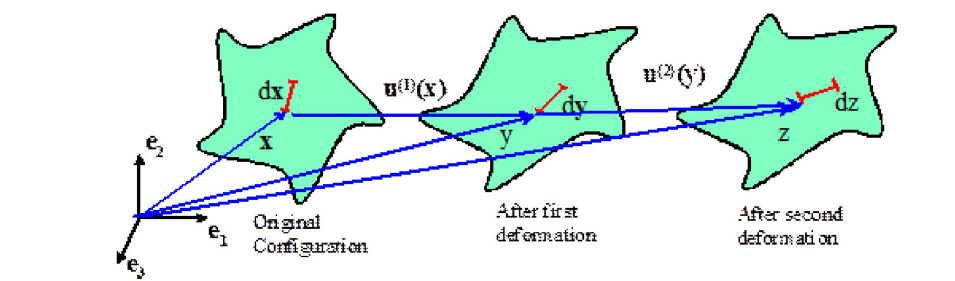
\includegraphics[scale=0.5]{../pictures/2-3/2-deformation.png}
\end{figure}
\end{frame}

\begin{frame}{Deformation gradient resulting from two successive deformations (2/3)}
\begin{itemize}
    \item \textbf{Deformation Gradients:}
        \begin{itemize}
            \item   $F^{(1)}$ and $F^{(2)}$ are deformation gradients:
                \[
                 F^{(1)} = y \otimes \nabla_x, \quad F^{(2)} = z \otimes \nabla_y
                \]
            \item   In component form:
                 \[
                 F_{ij}^{(1)} = \frac{\partial y_i}{\partial x_j}, \quad F_{ij}^{(2)} = \frac{\partial z_i}{\partial y_j}
                 \]
        \end{itemize}
\end{itemize}
\end{frame}

\begin{frame}{Deformation gradient resulting from two successive deformations (3/3)}
\begin{itemize}
    \item \textbf{Cumulative Deformation Gradient:}
        \begin{itemize}
            \item   The deformation gradient $F$ that maps $dx$ directly to $dz$ is:
                \[
                dz = F \cdot dx \quad \text{with} \quad F = F^{(2)} \cdot F^{(1)}
                \]
            \item   In component form:
                \[
                dz_i = F_{ij} dx_j, \quad F_{ij} = F_{ik}^{(2)} F_{kj}^{(1)}
                \]
        \end{itemize}
    \item \textbf{Chain Rule Application:}
        \begin{itemize}
            \item   The cumulative mapping can be written as $z_i(y_j(x_k))$.
            \item   Applying the chain rule:
                \[
                dz_i = \frac{\partial z_i}{\partial y_j} \frac{\partial y_j}{\partial x_k} dx_k
                \]
        \end{itemize}
\end{itemize}

\end{frame}

\begin{frame}{The Jacobian of the deformation gradient (1/4)}
\begin{itemize}
    \item \textbf{Definition:} The Jacobian of the deformation gradient is:
        \[
        J = det(F) = det\left(\delta_{ij} + \frac{\partial u_i}{\partial x_j}\right)
        \]
    \item \textbf{Volume Change:** $J$ measures the volume change due to deformation}.
\end{itemize}
\begin{figure}
    \centering
    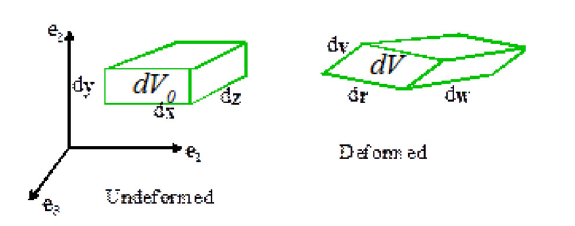
\includegraphics[scale=0.7]{../pictures/2-3/jacobian-deformation.png}
\end{figure}
\end{frame}

\begin{frame}{The Jacobian of the deformation gradient (2/4)}
\begin{itemize}
        \item \textbf{Infinitesimal Volume Element:}
        \begin{itemize}
            \item   Consider an infinitesimal volume element with sides $dx$, $dy$, and $dz$.
            \item   Original volume: $dV_0 = dz \cdot (dx \times dy) = \epsilon_{ijk} dz_i dx_j dy_k$
        \end{itemize}
    \item \textbf{Deformed Volume Element:}
        \begin{itemize}
            \item   The element is mapped to a parallelepiped with sides $dr$, $dv$, and $dw$.
            \item   Deformed volume: $dV = \epsilon_{ijk} dw_i dr_j dv_k$
        \end{itemize}
    \item \textbf{Relationship between deformed and undeformed elements:}
         \begin{itemize}
            \item   $dr_i = F_{il} dx_l$,  $dv_j = F_{jm} dy_m$,  $dw_k = F_{kn} dz_n$
         \end{itemize}
\end{itemize}
\end{frame}

\begin{frame}{The Jacobian of the deformation gradient (3/4)}
\begin{itemize}
    \item \textbf{Volume Transformation:}
        \begin{itemize}
            \item   $dV = \epsilon_{ijk} F_{il} F_{jm} F_{kn} dx_l dy_m dz_n$
            \item   Using the identity $\epsilon_{ijk} A_{il} A_{jm} A_{kn} = \epsilon_{lmn} det(A)$:
                \[
                dV = det(F) \epsilon_{lmn} dx_l dy_m dz_n = det(F) dV_0
                \]
        \end{itemize}
    \item \textbf{Volume Ratio:}
        \begin{itemize}
            \item   The ratio of deformed to undeformed volume:
                \[
                \frac{dV}{dV_0} = det(F) = J
                \]
        \end{itemize}
    \item \textbf{Physical Admissibility:} For any physically admissible deformation, $J > 0$.
    \item \textbf{Incompressibility:} For incompressible materials, $J = 1$.
    \item \textbf{Density Transformation:} Mass density transforms as $\rho = \frac{\rho_0}{J}$.
\end{itemize}
\end{frame}

\begin{frame}{The Jacobian of the deformation gradient (4/4)}
\begin{itemize}
    \item \textbf{Jacobian Derivative:} Derivative of J with respect to F:
        \[
        \frac{\partial J}{\partial F_{ij}} = J F_{ji}^{-1}
        \]
\end{itemize}
\end{frame}

  \end{document}